\section{Magnetiskt fält}
\textbf{HAREC a.\ref{HAREC.a.1.4}\label{myHAREC.a.1.4}}
\label{elektromagnetiskafält}
\index{elektromagnetiska fält}

\subsection{Magnetism}
\index{magnetism}
\index{Plinius}
\index{Magnes}
\index{Lithos herakleia}
\index{Herakleia}
\index{Magnesia}
\index{Magnetes}

\infobox{
Enligt den romerske författaren \emph{Plinius} lär, vid tiden ungefär
160 år f. K. herden \emph{Magnes} en dag ha känt hur järnstiften i
sandalerna häftade vid en viss sorts sten. Det kunde ha varit
svart järnmalm, som grekerna i äldsta tider benämnde
\emph{Lithos herakleia} efter staden \emph{Herakleia} i Lydien,
där sådan malm förekommer. Staden fick sedermera namnet
\emph{Magnesia} och man kan tänka sig att stenen kom att kallas
\emph{Magnetes}. En hel mineralgrupp med liknande egenskaper,
såsom järn, nickel m. fl. kallas magnetiska.
}

\emph{Magnetism} uppstår av elektriska laddningar i rörelse. Elektronernas rörelser i
en atom skapar nämligen magnetfält. Det gör att atomerna var för sig fungerar
som en magnetisk dipol - en magnet. I de flesta material är atomerna
orienterade så att deras magnetiska krafter tar ut varandra. Materialet som
helhet är då omagnetiskt och utövar inga yttre krafter. Men vid påverkan från
ett yttre magnetfält kan dipolerna (atomerna) i ett material orienteras i samma
riktning och deras magnetfält kommer då att samverka. Hela materialet blir då
magnetiskt. När det yttre magnetfältet avlägsnas, kvarstår orienteringen endast
delvis - \emph{magnetisk remanens}. I ferromagnetiska legeringar kvarstår en
större del av orienteringen, även om påverkan från det yttre magnetfältet har
upphört. Materialet är då permanentmagnetiskt.

\subsection{Kraftfält i och omkring magneter}

\begin{figure*}
  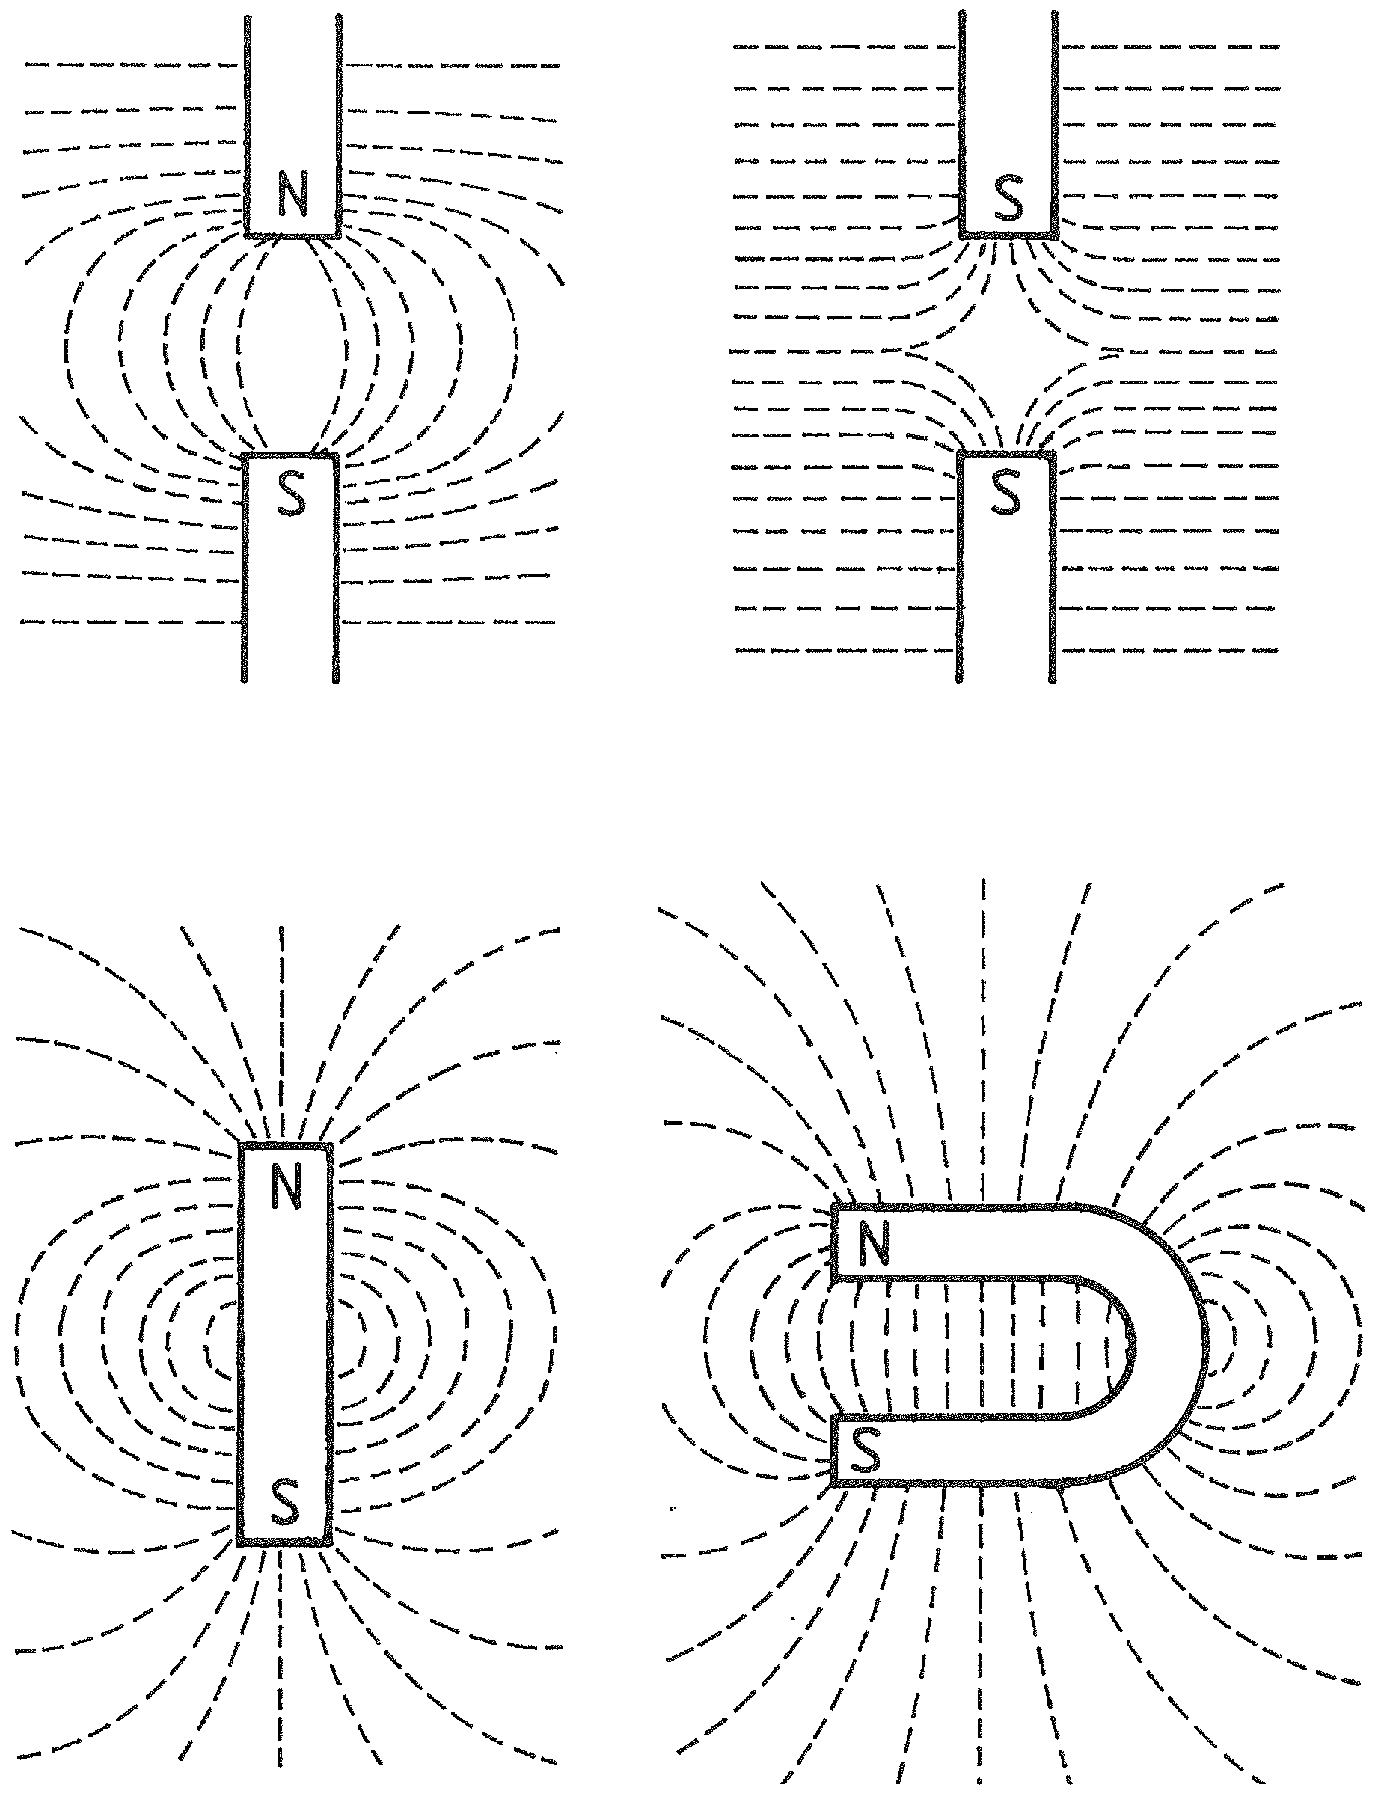
\includegraphics[width=\textwidth]{images/bild_2_1-07}
  \caption{Kraftfält omkring magneter}
  \label{fig:BildII1-7}
\end{figure*}

Bild \ref{fig:BildII1-7}.

Varje magnet omges av ett magnetiskt kraftfält. Magnetfältets fördelning,
styrka och riktningar beskrivs som kraftlinjer med slutna kretslopp.

Utanför magneten går kraftlinjerna från nord- till sydpol och inne i magneten 
motsatt riktning. Kraftriktningen i varje punkt av fältet är den som nordändan
på en kompassnål skulle peka åt. Om man hänger upp en magnet i en tråd, så
kommer den att inta samma riktning som jordens magnetfält.

\begin{quote}
\emph{Poler med samma polaritet stöter bort varandra (repellerar).}

\emph{Poler med olika polaritet dras till varandra (attraherar).}
\end{quote}

\subsection{Magnetiska fält omkring strömbanor}
\textbf{HAREC a.\ref{HAREC.a.1.4.1}\label{myHAREC.a.1.4.1}}

\begin{figure*}
  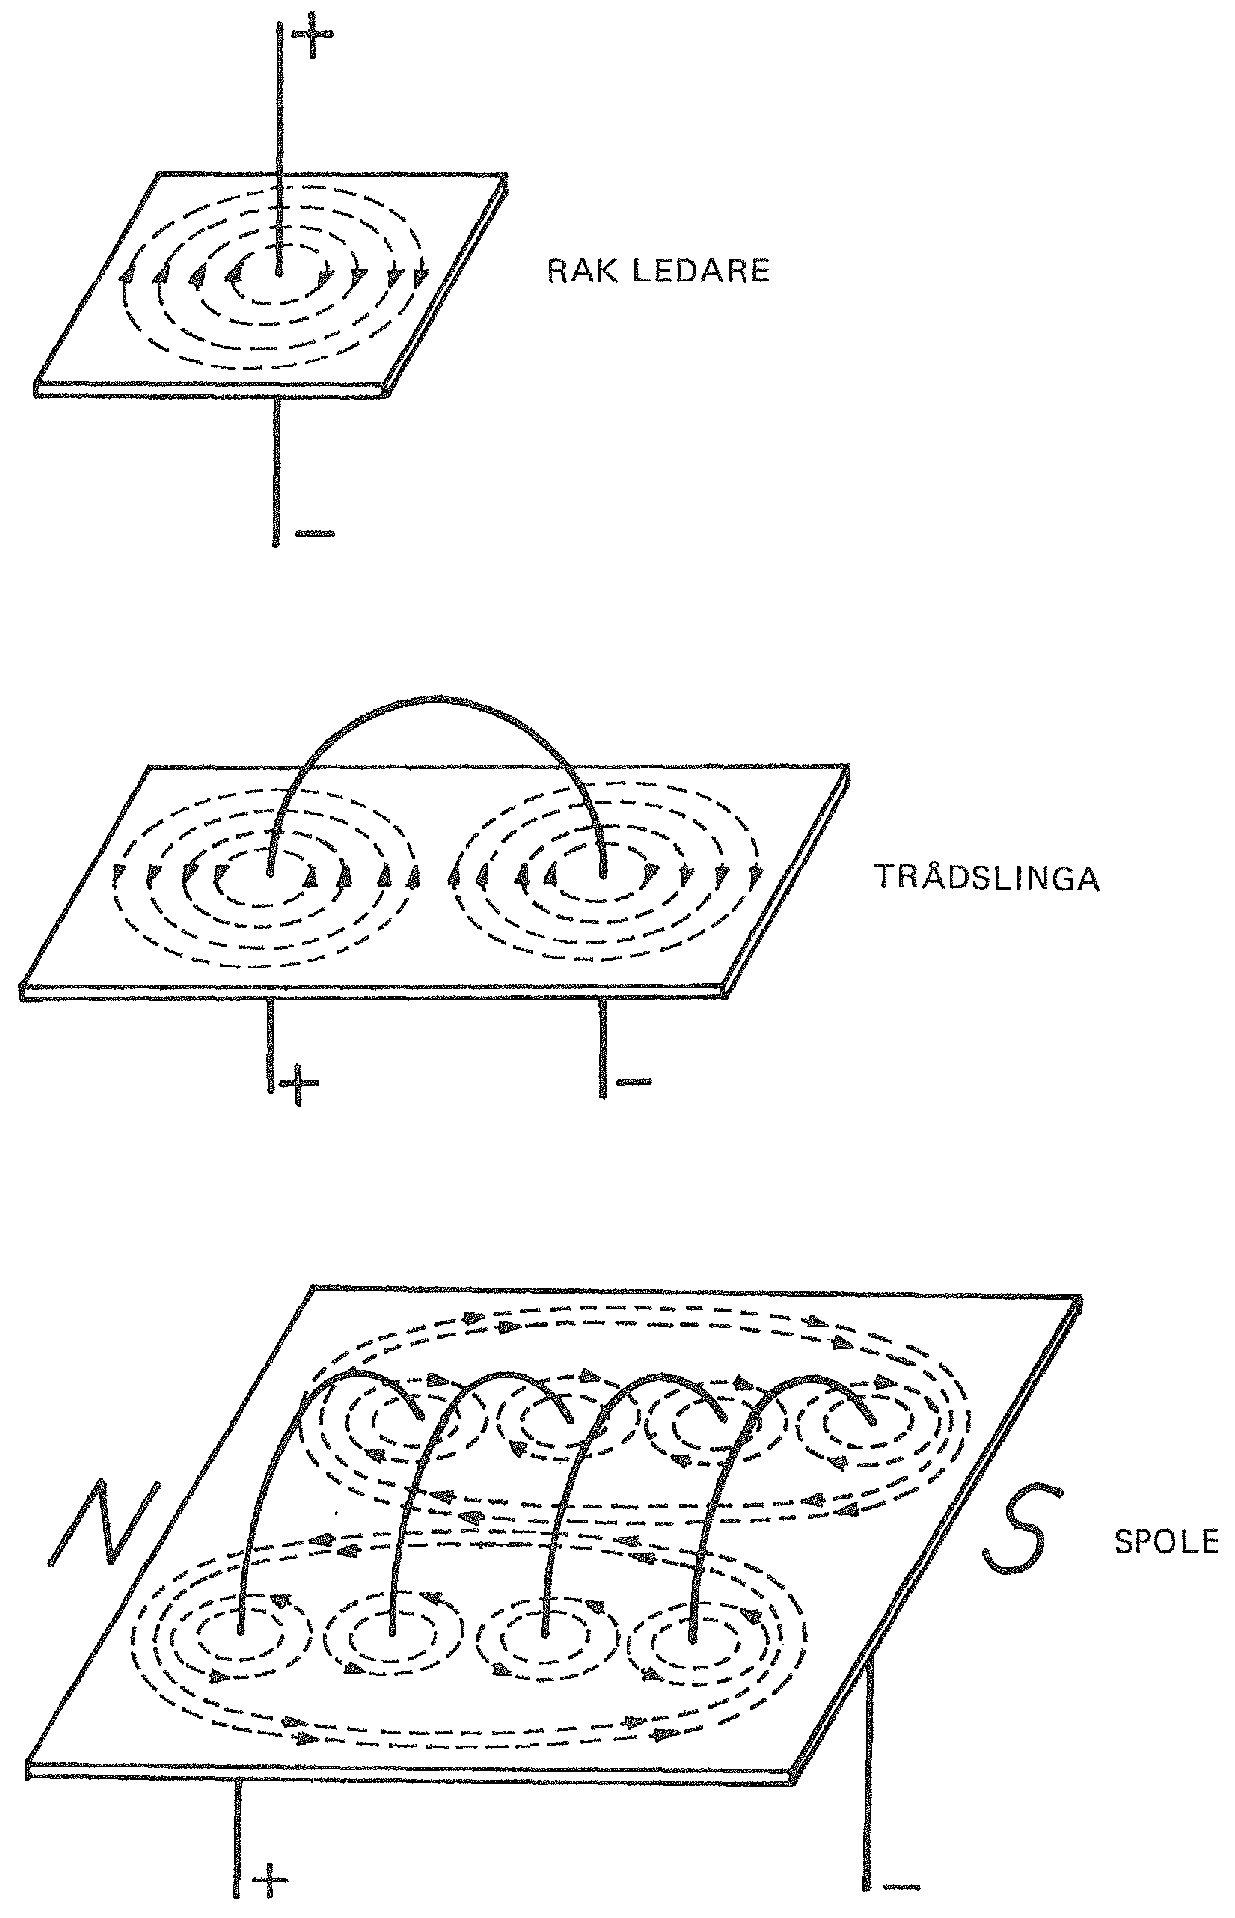
\includegraphics[width=\textwidth]{images/bild_2_1-08}
  \caption{Magnetiska fält omkring strömledare}
  \label{fig:BildII1-8}
\end{figure*}

Bild \ref{fig:BildII1-8}.

Omkring varje ledare, som det flyter en elektrisk ström igenom, alstras det ett
magnetiskt kraftfält.

Magnetiska kraftlinjerna fördelar sig koncentriskt omkring en rak ledare och
vinkelrätt mot denna.

Mellan ändarna av en ledare med bågformad utsträckning bildas kraftlinjer som
verkar med varandra.

En strömgenomfluten cylindrisk spole - induktor - uppvisar samma magnetiska
fältbild som en stavformad permanentmagnet.

\subsection{Bestämma magnetiska fältriktningen}

Magnetfältets riktning omkring en ledare kan enkelt bestämmas med
\emph{högerhandsregeln}
\url{https://sv.wikipedia.org/wiki/Högerhandsregeln}.

När en \emph{ledare} fattas med höger hand och med tummen i strömmens
riktning, så kommer fingrarna att peka i fältriktningen (B).

I bild \ref{fig:BildII1-8} (övre) så går strömmen från pluspolen (+) till
minuspolen (-) varvid strömmen komme gå nedåt i bilden på ovansidan,
dvs. precis så tummen pekar om man greppar ledaren med tummen nedåt, och
magnetfältet kommer snurra som pilarna precis som de övriga fingrarna på
högerhanden.

När en ledare formas som en spole och en elektrisk ström flyter genom den,
kommer magnetfältet att ha ett utseende som liknar det omkring en
permanentmagnet.

En sådan spole kallas \emph{elektromagnet}.

Magnetfältets riktning i en spole kan också bestämmas med högerhandsregeln.
När \emph{en spole} fattas med höger hand och med fingrarna i strömmens
riktning, så kommer den utsträckta tummen att peka mot spolens nordpol.

I bild \ref{fig:BildII1-8} (undre) så går strömmen från pluspolen (+) till minuspolen
(-) varvid strömmen kommer gå inåt i bilden på ovansidan, dvs. precis så
fingrarna pekar när man lägger handen på spolen, och magnetfältet kommer peka
mot nord (N) precis som tummen på högerhanden.

Fälten omkring alla slags magneter, såväl permanentmagnetiska som elektromag-
netiska, återverkar på varandra. Även enkla
elektriska ledare är elektromagneter.

\clearpage

\subsection{Exempel på elektromagneter}

\begin{wrapfigure}{r}{0.5\textwidth}
  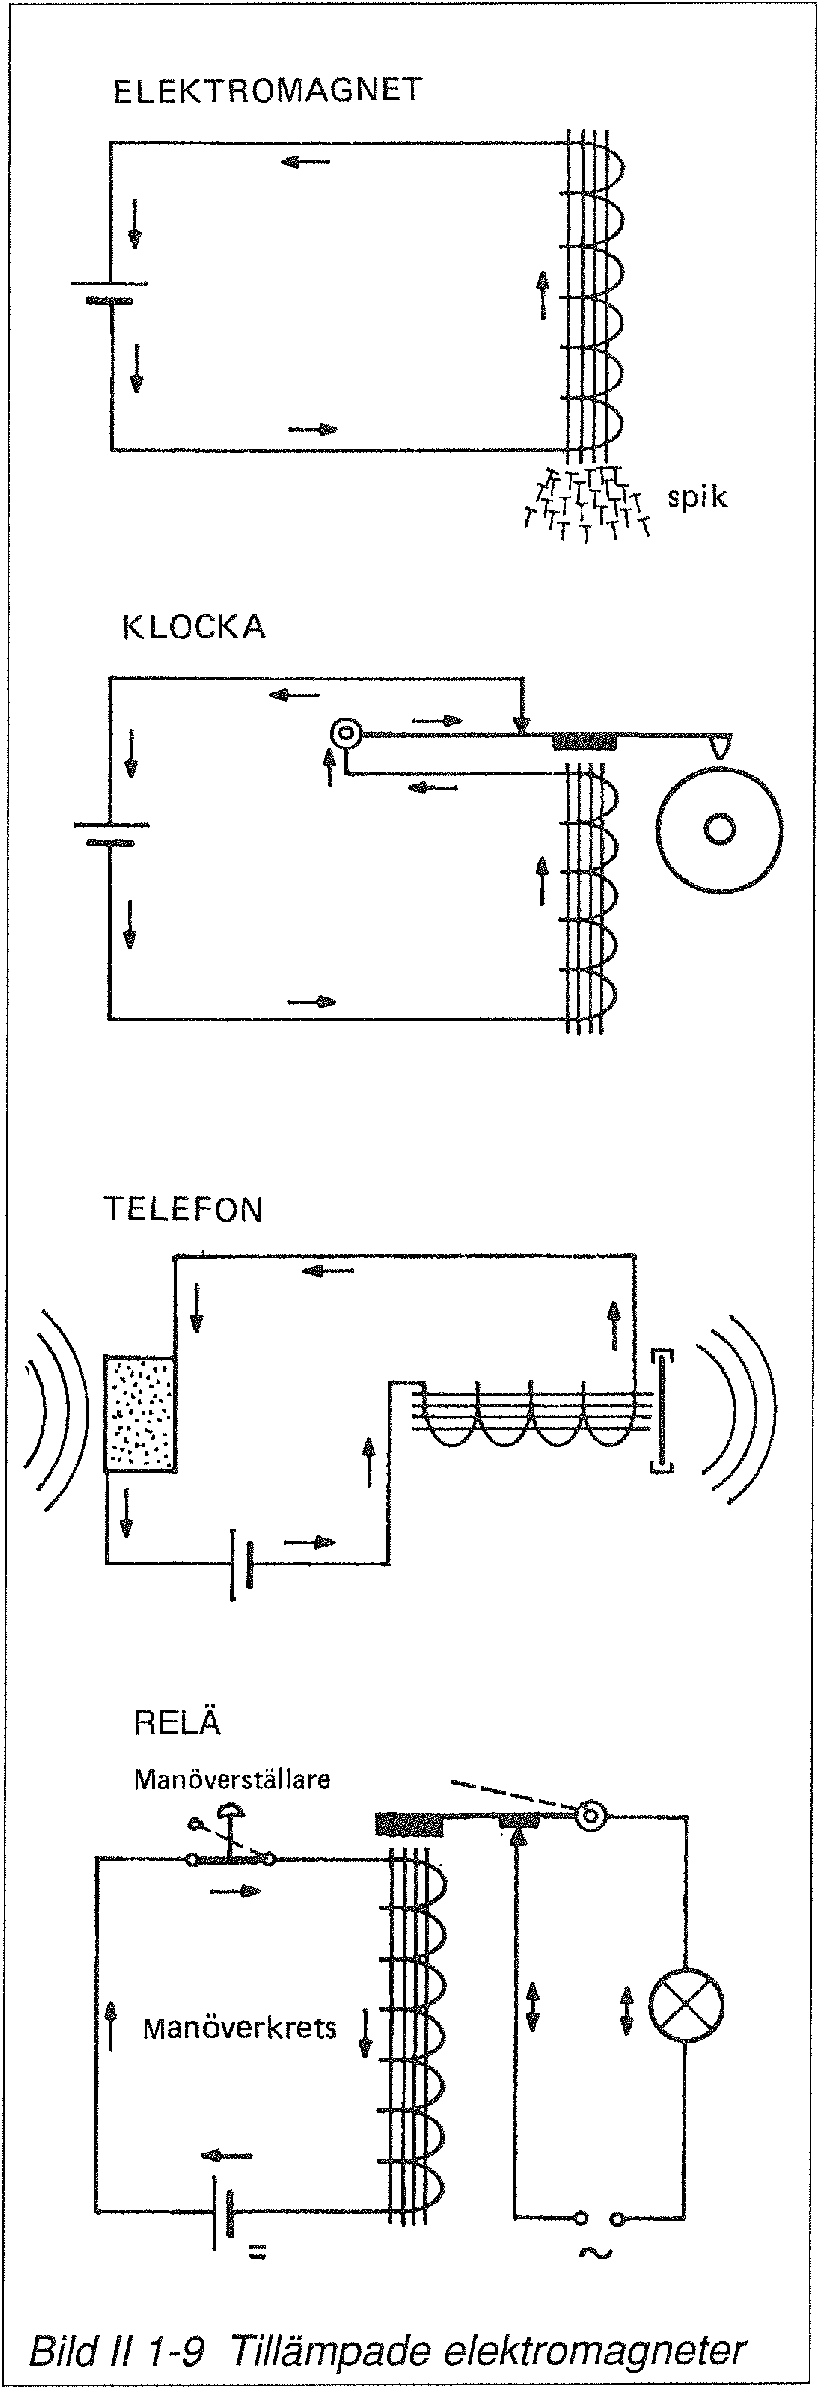
\includegraphics[width=0.5\textwidth]{images/bild_2_1-09}
  \caption{Exempel på elektromagneter}
  \label{fig:BildII1-9}
\end{wrapfigure}

Bild \ref{fig:BildII1-9}.

\subsubsection{Elektromagnet}
Det bildas ett magnetfält genom en spole så länge som det flyter ström genom
den. En järnkärna i spolen koncentrerar fältet p.g.a. den större magnetiska
ledningsförmågan.

Elektromagneter används för att sätta magnetiska material i rörelse eller hålla
fast dem.

\subsubsection{Elektrisk ringklocka}
Anordningen består av en elektromagnet och en järnplatta på en fjäder. På plattan
sitter en självbrytande kontakt samt en kläpp som kan slå på en klocka.

Kontakten åstadkommer en växelvis brytning och slutning av strömmen genom
elektromagneten. Armaturen med kläppen kommer då i svängning och slår på
klockan.

\subsubsection{Telefon}
I en enkel telefon finns bl.a. en mikrofon, ett batteri och en hörtelefon.

Särskilt i äldre telefoner består mikrofonen av en kolkornskammare med ett
membran. Trycksvariationer (ljud) får membranet att vibrera, varvid resistansen
genom kolkornen varierar i motsvarande grad. Därmed varierar talströmmen genom
mikrofonen.

Hörtelefonen består av en elektromagnet och ett membran av mjukjärn.
Variationer i talströmmen genom mikrofonen passerar även hörtelefonen får dess
magnetfält att variera. Hörtelefonens membran alstrar då trycksvariationer,
d.v.s. ljud.

\subsubsection{Elektromagnetiskt relä}
Reläet består av en elektromagnet, en järnplatta (ankare) på en fjäder och en
elektrisk kontakt. Med en svag ström / låg spänning genom spolen i
manöverkretsen, så kan man med reläets arbetskontakt styra starkare ström / högre
spänning i huvudkretsen.

\subsection{Magnetisk fältstyrka}
\index{magnetisk fältstyrka}
\index{symbol!\(H\) magnetisk fältstyrka}

Som magnetisk fältstyrka förstår man flödet per meter fältlinje, d.v.s.

\begin{align*}
  &H = \frac{\Theta}{l} = \frac{I \cdot N}{l} \\
  &H\ [A/m] \\
  &I\ [A] \\
  &N\ \text{[varvtal]} \\
  &l\ \text{[fältlinjelängd]}
\end{align*}

\emph{Magnetisk fältstyrka uttrycks således som Ampere per meter flödesväg.}

\subsection{Magnetisk flödestäthet}
\index{magnetisk flödestäthet}
\index{Tesla (T)}
\index{enheter!Tesla (T)}
\index{symbol!\(B\) magnetisk flödestäthet}
\index{permabilitet}
\index{symbol!\(\mu\) permabilitet}

\emph{Den magnetiska flödestätheten mäts i enheten Tesla \([T]\) (förut Gauss).}

Formeltecknet/symbol är \(B\).

Formeln är \(B = \mu \cdot H\)

Flödestäthet \(B\ [Vs/m^2]\) Fältstyrka \(H\ [A/m]\)

\(\mu\) är permabilitetstalet för materialet.
\(\mu_0\) är permeabilitetstalet (fältkonstanten) för den magnetiska
ledningsförmåga för luft och omagnetiska material.

För järn eller annat magnetiskt ledande material tillkommer permeabilitetstalet
\(\mu_r\). Det anger hur många gånger bättre än luft etc., som materialet det
leder ett magnetisk flöde. Permabilitetstalet kan då skrivas
\(\mu = \mu_r\mu_0\).

Formeln är \(B = \mu_0 \cdot \mu_r \cdot H\)

\subsection{Magnetiskt flöde}
\index{magnetiskt flöde}
\index{symbol!\(\Phi\) magnetiskt flöde}

Det magnetiska flödet är produkten avflödestätheten \(B\) och tvärsnittsytan
\(A\) av flödesvägen, således

\(\Phi = B \cdot A\)

\(\Phi \text{[Weber eller Vs]}\) \(B \text{[T eller Tesla]}\) \(A [m^2]\)

\subsection{Skärmning av magnetiska fält}
\textbf{HAREC a.\ref{HAREC.a.1.4.2}\label{myHAREC.a.1.4.2}}
\index{magnetiska fält!skärmning}
\label{elektromagnetisk skärmning}

I grunden finns det två slags fält, det elektriska och det magnetiska. Det
finns även elektromagnetiska fält, som är sammansatt av båda dessa. Fält kan
vara permanenta eller rörliga, varav här avses de rörliga. Ett rörligt
magnetiskt fält genererar ett elektriskt fält. Omvänt generar ett rörligt
elektriskt fält ett rörligt magnetiskt fält. Denna växelverkan gör att fälten
kan hållas igång med tillförsel av yttre energi.

Fält i rörelse alstrar elektromagnetisk strålning, som påverkar funktioner i
omgivningen. När påverkan inte är önskvärd, måste fältet skärmas av. Ett sätt
att skärma magnetiska fält är en metallisk kapsling. Kapslingen skall vara tät
och bilda en sluten magnetisk krets. Kapslingen skall vara utförd i ett
material som är en god ledare av magnetiskt flöde.
(Jämför \ref{elektrostatik skärmning})
